\begin{exercise}
      {ID-bd2471708d3f765a90ce138637c8bf3e4703e586}
      {High Noon}
  \ifproblem\problem
    In den beiden Orten $A$ und $B$ brechen zur selben Zeit zwei Fahrradfahrer auf.
    Der Fahrradfahrer, der in $A$ startet, fährt nach $B$, und der Fahrradfahrer, der
    in $B$ startet, fährt nach $A$. Sie benutzen denselben Weg und treffen sich genau um
    12:00 Uhr mittags.
    \begin{center}
      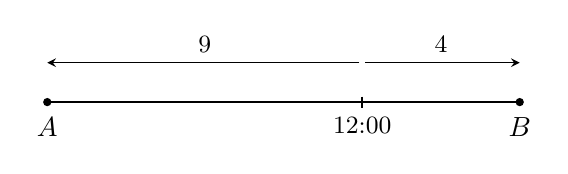
\begin{tikzpicture}
        % Weg
        \draw[line width=0.6pt] (0, 0) -- (6, 0);
        % Punkte
        \fill[fill=black] (0, 0) circle[radius=1.5pt] node[below=2pt]{$A$};
        \fill[fill=black] (6, 0) circle[radius=1.5pt] node[below=2pt]{$B$};
        % Markierung: 12:00
        \draw[line width=0.6pt] (4, 2pt) -- (4, -2pt) node[below]{\small12:00};
        % Pfeil: 9h
        \draw[line width=0.4pt, ->, >=stealth, shorten <=1pt]
             (4, 5mm) -- node[above]{\small\SI{9}{\hour}}
             (0, 5mm);
        % Pfeil: 4h
        \draw[line width=0.4pt, ->, >=stealth, shorten <=1pt]
             (4, 5mm) -- node[above]{\small\SI{4}{\hour}}
             (6, 5mm);
      \end{tikzpicture}
    \end{center}
    Nachdem sie sich begegnet sind, braucht der eine Fahrradfahrer noch 4
    Stunden bis er in $B$, und der andere Fahrradfahrer noch 9 Stunden bis
    er in $A$ angekommen ist. Wann sind die beiden Fahrradfahrer aufgebrochen?
  \fi
  %\ifoutline\outline
  %\fi
  %\ifoutcome\outcome
  %\fi
\end{exercise}
